% ═══════════════════════════════════════════════════════════════════════
%  Dissertation Presentation — LaTeX Beamer
%  Replicates the structure & style of Dissertation_template.pptx
%  "Prediction and Prevention of Diabetes using Explainable AI"
%  Tanya Singh  |  215/ICS/030  |  Gautam Buddha University
% ═══════════════════════════════════════════════════════════════════════
\documentclass[aspectratio=169, 11pt]{beamer}

% ── Packages ──────────────────────────────────────────────────────────
\usepackage[T1]{fontenc}
\usepackage{helvet}                       % Arial-like sans-serif
\renewcommand{\familydefault}{\sfdefault}
\usepackage{graphicx}
\usepackage{booktabs}
\usepackage{tabularx}
\usepackage{array}
\usepackage{amsmath}
\usepackage{multirow}
\usepackage{tikz}
\usepackage{xcolor}
\usepackage{calc}
\usepackage{hyperref}
\usepackage{ragged2e}
\usepackage{colortbl}

% ── Color Palette (from PPTX Office theme) ───────────────────────────
\definecolor{accent1}{HTML}{4472C4}       % Blue (primary accent)
\definecolor{accent3}{HTML}{A5A5A5}       % Gray (header bar)
\definecolor{dk2}{HTML}{44546A}           % Dark blue-gray
\definecolor{subtitleblue}{HTML}{3333FF}  % Subtitle text color
\definecolor{headertext}{HTML}{FFFFFF}    % White text on header
\definecolor{bodygray}{HTML}{7F7F7F}      % Body text gray
\definecolor{lightbg}{HTML}{F2F2F2}       % Light background accent
\definecolor{tabhead}{HTML}{4472C4}       % Table header blue
\definecolor{blockbg}{HTML}{DAE3F3}       % Block background light blue

% ── Global Spacing ───────────────────────────────────────────────────
\setlength{\parskip}{0pt}
\setlength{\parindent}{0pt}

% ── Beamer Theme Setup ───────────────────────────────────────────────
\usetheme{default}
\usecolortheme{default}
\setbeamercolor{background canvas}{bg=white}
\setbeamercolor{normal text}{fg=black}
\setbeamercolor{frametitle}{fg=dk2}
\setbeamercolor{item}{fg=accent1}
\setbeamercolor{subitem}{fg=dk2}
\setbeamercolor{itemize item}{fg=accent1}
\setbeamercolor{itemize subitem}{fg=dk2}
\setbeamercolor{enumerate item}{fg=accent1}
\setbeamercolor{enumerate subitem}{fg=dk2}
\setbeamertemplate{itemize item}{\small$\bullet$}
\setbeamertemplate{itemize subitem}{\scriptsize$\circ$}
\setbeamertemplate{enumerate items}[default]
\setbeamertemplate{navigation symbols}{}
\setbeamercolor{block title}{fg=white, bg=accent1}
\setbeamercolor{block body}{bg=blockbg}
\setbeamerfont{block title}{size=\small, series=\bfseries}
\setbeamerfont{block body}{size=\small}
\setbeamerfont{frametitle}{size=\large, series=\bfseries}

% ── Header Bar (top strip with logo + GBU text) ─────────────────────
\setbeamertemplate{headline}{%
  \begin{tikzpicture}[remember picture, overlay]
    \fill[accent3] (0, 0) rectangle (\paperwidth, 0.55cm);
    \node[anchor=west, inner sep=0pt] at (0.2cm, 0.275cm) {%
      \includegraphics[height=0.4cm]{Assets/gbulogo.pdf}%
    };
    \node[anchor=center, text=white, font=\tiny\bfseries] at (0.5\paperwidth, 0.275cm) {%
      Gautam Buddha University \textbar\ School of ICT%
    };
    \node[anchor=east, text=white, font=\tiny] at (\paperwidth-0.2cm, 0.275cm) {%
      \insertframenumber/\inserttotalframenumber%
    };
  \end{tikzpicture}%
  \vspace{0.55cm}%
}

% ── Footline ─────────────────────────────────────────────────────────
\setbeamertemplate{footline}{%
  \begin{tikzpicture}[remember picture, overlay]
    \draw[accent3, line width=0.4pt] (0.5cm, 0.35cm) -- (\paperwidth-0.5cm, 0.35cm);
    \node[anchor=west, font=\tiny, text=bodygray] at (0.5cm, 0.13cm) {February 2026};
    \node[anchor=center, font=\tiny, text=bodygray] at (0.5\paperwidth, 0.13cm) {Dissertation Presentation --- Tanya Singh};
    \node[anchor=east, font=\tiny, text=bodygray] at (\paperwidth-0.5cm, 0.13cm) {\insertframenumber/\inserttotalframenumber};
  \end{tikzpicture}%
  \vspace{0.4cm}%
}

% ── Frame Title ─────────────────────────────────────────────────────
\setbeamertemplate{frametitle}{%
  \vspace{0.05cm}%
  \noindent\textcolor{dk2}{\large\bfseries\insertframetitle}%
  \vspace{0.05cm}%
  \par\noindent\textcolor{accent1}{\rule{\textwidth}{0.6pt}}%
  \vspace{-0.1cm}%
}

% ── Section slide command (SECTION_HEADER layout) ────────────────────
\newcommand{\sectionslide}[2]{%
  {%
  \setbeamertemplate{headline}{}%
  \setbeamertemplate{footline}{%
    \begin{tikzpicture}[remember picture, overlay]
      \node[anchor=east, font=\tiny, text=bodygray] at (\paperwidth-0.5cm, 0.25cm) {\insertframenumber/\inserttotalframenumber};
    \end{tikzpicture}%
    \vspace{0.25cm}%
  }%
  \begin{frame}[plain]
    \begin{tikzpicture}[remember picture, overlay]
      % Header bar
      \fill[accent3] ([yshift=0cm]current page.north west) rectangle ([yshift=-0.55cm]current page.north east);
      \node[anchor=west, inner sep=0pt] at ([xshift=0.2cm, yshift=-0.275cm]current page.north west) {%
        \includegraphics[height=0.4cm]{Assets/gbulogo.pdf}%
      };
      \node[anchor=center, text=white, font=\tiny\bfseries] at ([yshift=-0.275cm]current page.north) {%
        Gautam Buddha University \textbar\ School of ICT%
      };
      \node[anchor=east, text=white, font=\tiny] at ([xshift=-0.2cm, yshift=-0.275cm]current page.north east) {%
        \insertframenumber/\inserttotalframenumber%
      };
      % Left accent stripe
      \fill[accent1] ([xshift=0cm, yshift=-1.8cm]current page.north west) rectangle ([xshift=0.35cm, yshift=-5.5cm]current page.north west);
    \end{tikzpicture}%

    \vspace{1.2cm}

    \hspace{0.6cm}{\fontsize{26}{32}\selectfont\textcolor{dk2}{\textbf{#1}}}

    \vspace{0.6cm}

    \hspace{0.8cm}{\normalsize\textcolor{bodygray}{#2}}
  \end{frame}
  }%
}

% ── Title slide command (TITLE layout) ───────────────────────────────
\newcommand{\titleslide}{%
  {%
  \setbeamertemplate{headline}{}%
  \setbeamertemplate{footline}{%
    \begin{tikzpicture}[remember picture, overlay]
      \node[anchor=west, font=\tiny, text=bodygray] at (0.5cm, 0.25cm) {February 2026};
      \node[anchor=center, font=\tiny, text=bodygray] at (0.5\paperwidth, 0.25cm) {Dissertation Presentation};
      \node[anchor=east, font=\tiny, text=bodygray] at (\paperwidth-0.5cm, 0.25cm) {1/\inserttotalframenumber};
    \end{tikzpicture}%
    \vspace{0.25cm}%
  }%
  \begin{frame}[plain]
    \begin{tikzpicture}[remember picture, overlay]
      \fill[accent3] ([yshift=0cm]current page.north west) rectangle ([yshift=-0.12cm]current page.north east);
    \end{tikzpicture}%

    \vspace{-0.3cm}

    \begin{center}
      \includegraphics[height=1.1cm]{Assets/gbulogo.pdf}

      \vspace{0.05cm}
      {\small School of Information and Communication Technology}

      \vspace{0.25cm}
      {\fontsize{19}{24}\selectfont\textcolor{dk2}{\textbf{Prediction and Prevention of Diabetes\\[3pt] using Explainable AI}}}

      \vspace{0.2cm}
      {\normalsize\textcolor{subtitleblue}{Dissertation Presentation}}
    \end{center}

    \vspace{0.25cm}

    \begin{columns}[T]
      \begin{column}{0.45\textwidth}
        \begin{center}
          {\small\textbf{Under Supervision of:}}\\[2pt]
          {\small Dr.\ Rakesh Kumar}\\
          {\footnotesize Assistant Professor, Dept.\ of CSE}
        \end{center}
      \end{column}
      \hfill
      \begin{column}{0.45\textwidth}
        \begin{flushright}
          {\small\textbf{Tanya Singh}}\\[2pt]
          {\small Roll No: 215/ICS/030}\\
          {\footnotesize Int.\ B.Tech.\ + M.Tech\ (CSE -- Data Science)}
        \end{flushright}
      \end{column}
    \end{columns}
  \end{frame}
  }%
}

% ═══════════════════════════════════════════════════════════════════════
%  DOCUMENT
% ═══════════════════════════════════════════════════════════════════════
\begin{document}

% =====================================================================
%  SLIDE 1 — Title
% =====================================================================
\titleslide

% =====================================================================
%  SLIDE 2 — Outline
% =====================================================================
\begin{frame}{Outline of the Presentation}
  \vspace{0.3cm}
  \begin{enumerate}
    \setlength{\itemsep}{10pt}
    \item[\textcolor{accent1}{\textbf{1.}}] \textbf{Introduction} --- Research Area \& Problem Statement
    \item[\textcolor{accent1}{\textbf{2.}}] \textbf{Background} --- Literature Review, Research Gaps \& Objectives
    \item[\textcolor{accent1}{\textbf{3.}}] \textbf{Methodology} --- Dataset, Feature Engineering, Ensemble Architecture
    \item[\textcolor{accent1}{\textbf{4.}}] \textbf{Results \& Discussion} --- Multi-Threshold Performance, Cross-Validation
    \item[\textcolor{accent1}{\textbf{5.}}] \textbf{Conclusion} --- Key Findings, Limitations \& Future Work
    \item[\textcolor{accent1}{\textbf{6.}}] \textbf{References}
  \end{enumerate}
\end{frame}

% =====================================================================
%  SLIDE 3 — Section Header: Introduction
% =====================================================================
\sectionslide{Introduction}{%
  \\[4pt]
  
}

% =====================================================================
%  SLIDE 4 — Research Area
% =====================================================================
\begin{frame}{Research Area}
  \small
  \begin{itemize}
    \setlength{\itemsep}{7pt}
    \item Type~2 Diabetes Mellitus (T2DM) affects \textbf{537 million} adults globally, projected to reach \textbf{783 million} by 2045
    \item Early identification through non-invasive screening is critical yet underserved
    \item AI and Machine Learning show strong efficacy for diabetes risk assessment using epidemiological datasets
    \item Gradient-boosted methods (XGBoost, LightGBM, CatBoost) consistently outperform traditional classifiers
    \item \textbf{Explainable AI (XAI)} is essential for clinical trust --- SHAP, LIME, counterfactual explanations
    \item Key challenge: bridging the gap between \textbf{research prototypes} and \textbf{deployable clinical systems}
  \end{itemize}
\end{frame}

% =====================================================================
%  SLIDE 5 — Problem Statement
% =====================================================================
\begin{frame}{Problem Statement}
  \small
  \begin{enumerate}
    \setlength{\itemsep}{8pt}
    \item Most approaches use a \textbf{single binary threshold} (HbA1c~$\geq$~5.7\%), ignoring clinical heterogeneity of screening scenarios
    \item Few systems combine \textbf{per-patient SHAP explanations} with \textbf{actionable counterfactual} recommendations for lifestyle changes
    \item Persistent \textbf{translation gap} between research prototypes and production-grade clinical systems --- lacking fairness monitoring, deployment architecture
    \item No empirical study on the \textbf{impact of target threshold definition} on model performance has been reported
  \end{enumerate}
\end{frame}

% =====================================================================
%  SLIDE 6 — Section Header: Background
% =====================================================================
\sectionslide{Background}{%
  \\[4pt]
  \\[4pt]
 %
}

% =====================================================================
%  SLIDE 7 — Literature Review
% =====================================================================
\begin{frame}{Literature Review}
  \vspace{-0.1cm}
  \renewcommand{\arraystretch}{1.1}
  \centering
  \footnotesize
  \begin{tabularx}{0.98\textwidth}{|>{\raggedright\arraybackslash}p{2.1cm}|>{\raggedright\arraybackslash}p{2cm}|X|>{\raggedright\arraybackslash}p{1.8cm}|}
    \hline
    \rowcolor{accent1}\textcolor{white}{\textbf{Study}} & \textcolor{white}{\textbf{Method}} & \textcolor{white}{\textbf{Key Contribution}} & \textcolor{white}{\textbf{Limitation}} \\
    \hline
    Khokhar et al.\ '25 & Systematic review & Gradient-boosted methods outperform traditional classifiers & Single threshold \\
    \hline
    Nie et al.\ '24 & Deep learning & DRPM: 36$\to$5 features, strong AUC on NHANES & Limited features \\
    \hline
    Noh \& Kim '24 & GB + LiNGAM & Causal discovery, ${\sim}$84.8\% accuracy & No XAI layer \\
    \hline
    Shah et al.\ '25 & Hybrid ensemble & CVD risk, AUC\,=\,0.82, SHAP-based & Not diabetes-specific \\
    \hline
    Tasin et al.\ '23 & ML + XAI & SHAP + LIME for diabetes prediction & No counterfactuals \\
    \hline
    Maimaitijiang '25 & CatBoost + SHAP & Personalised chatbot assistant & Single model \\
    \hline
    Kabir et al.\ '25 & Counterfactual & Proximity-constrained counterfactuals & No SHAP \\
    \hline
    Mohanty et al.\ '25 & XAI + LLM & IMPACT: multi-disease prevention & Not diabetes-focused \\
    \hline
  \end{tabularx}
\end{frame}

% =====================================================================
%  SLIDE 8 — Research Gaps
% =====================================================================
\begin{frame}{Research Gaps}
  \small
  \vspace{0.1cm}
  \begin{description}
    \setlength{\itemsep}{10pt}
    \item[\textcolor{accent1}{Gap 1:}] \textbf{Single-threshold classification} --- majority of systems use only HbA1c~$\geq$~5.7\% without multi-threshold adaptability
    \item[\textcolor{accent1}{Gap 2:}] \textbf{Lack of integrated explainability} --- few combine per-patient SHAP explanations with actionable counterfactual interventions
    \item[\textcolor{accent1}{Gap 3:}] \textbf{Research-to-deployment gap} --- most systems lack production-grade architecture, fairness monitoring, or HIPAA compliance
    \item[\textcolor{accent1}{Gap 4:}] \textbf{No threshold impact study} --- no empirical analysis of how target threshold definition affects predictive performance
  \end{description}
\end{frame}

% =====================================================================
%  SLIDE 9 — Research Objectives
% =====================================================================
\begin{frame}{Research Objectives}
  \small
  \vspace{0.1cm}
  \begin{enumerate}
    \setlength{\itemsep}{7pt}
    \item \textbf{Multi-Threshold Ensemble Architecture:} Train three independent weighted-blend ensembles (LightGBM, CatBoost, XGBoost) for HbA1c thresholds $\geq$5.7\%, $\geq$5.9\%, $\geq$6.5\%
    \item \textbf{Target Threshold Dominance:} Empirically demonstrate that threshold choice is the single most impactful determinant of AUC (0.885~$\to$~0.972)
    \item \textbf{Multi-Modal Explainability:} SHAP waterfall + DiCE counterfactual interventions + WHO epidemiological cross-validation
    \item \textbf{Production-Grade Deployment:} Full-stack system --- FastAPI backend, Next.js~14 frontend, fairness auditing, HIPAA-compliant, containerised
  \end{enumerate}
\end{frame}

% =====================================================================
%  SLIDE 10 — Section Header: Methodology
% =====================================================================
\sectionslide{Methodology}{%
 
}

% =====================================================================
%  SLIDE 11 — Dataset
% =====================================================================
\begin{frame}{Dataset}
  \small
  \begin{columns}[T]
    \begin{column}{0.64\textwidth}
      \begin{itemize}
        \setlength{\itemsep}{4pt}
        \item \textbf{Source:} U.S.\ NHANES (National Health and Nutrition Examination Survey)
        \item \textbf{Span:} 12 survey cycles (1999--2024), 6 domains merged on SEQN
        \item \textbf{Records:} 67,876 $\to$ \textbf{33,333} (fasting glucose subsample)
        \item \textbf{Split:} 80/20 stratified (26,666 train / 6,667 test)
        \item \textbf{Features:} 62 total --- 23 base + 23 engineered + 16 missingness indicators
        \item \textbf{HbA1c excluded} from features (used as target); FastingGlucose is primary glycaemic predictor
      \end{itemize}
    \end{column}
    \begin{column}{0.44\textwidth}
      \centering
      \vspace{0.2cm}
      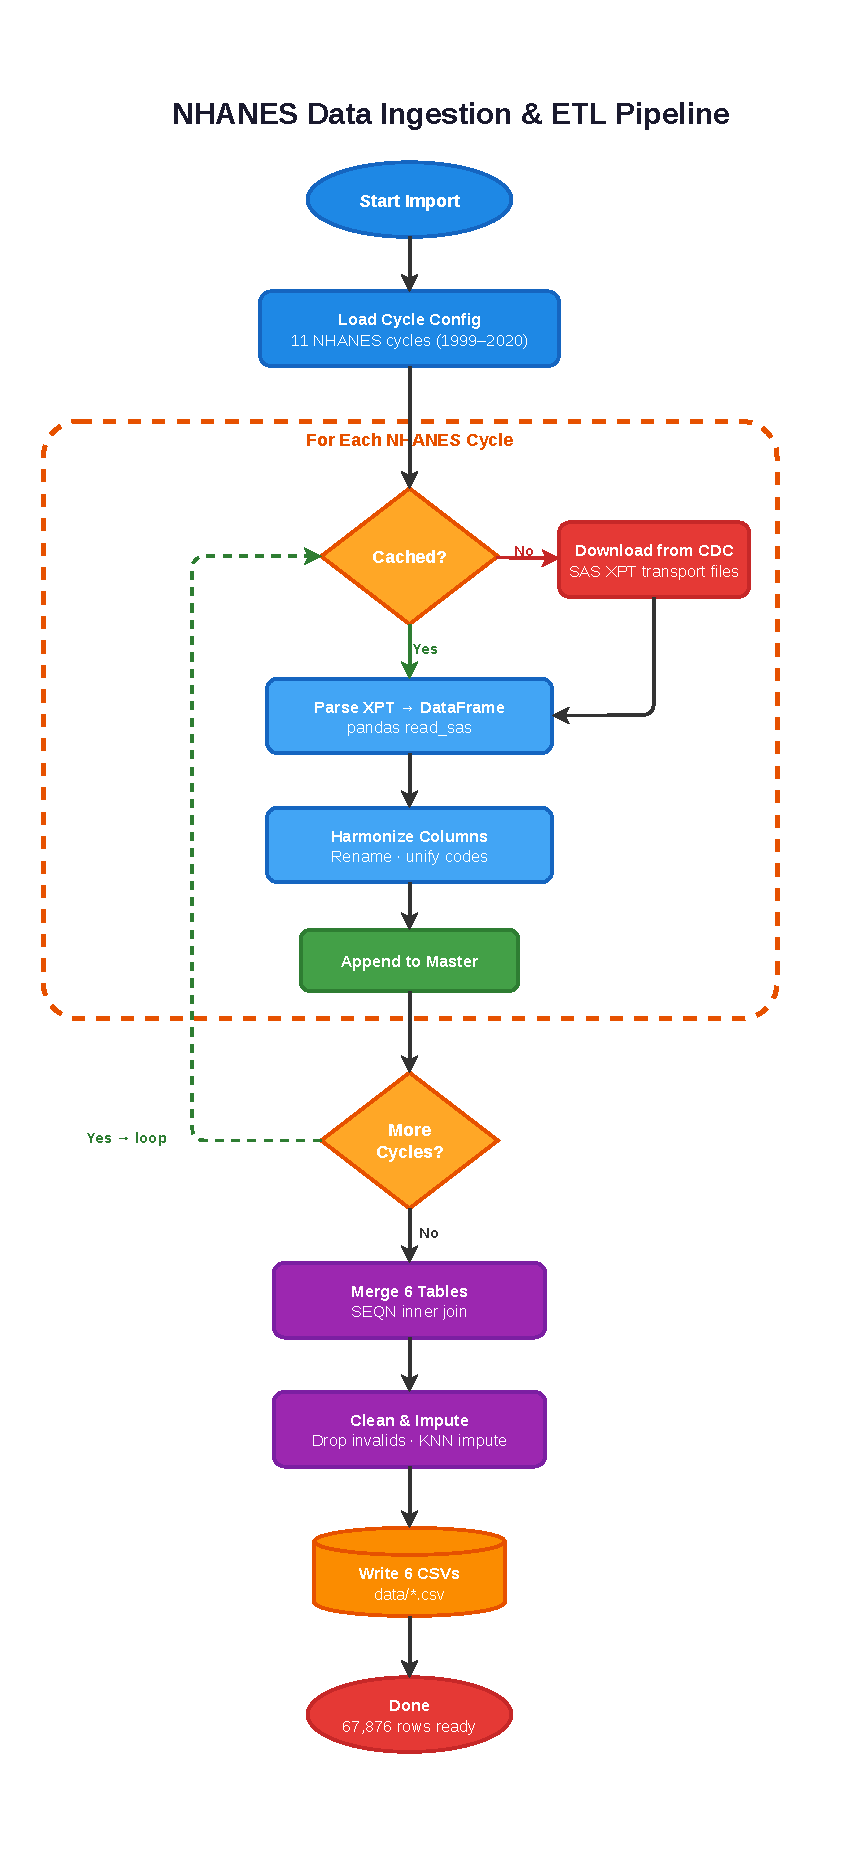
\includegraphics[width=0.92\linewidth, height=4.5cm, keepaspectratio]{Assets/nhanes_etl.pdf}

      \vspace{0.15cm}
      {\scriptsize\textcolor{bodygray}{NHANES Data Ingestion \& ETL Pipeline}}
    \end{column}
  \end{columns}
\end{frame}

% =====================================================================
%  SLIDE 12 — Methodology
% =====================================================================
\begin{frame}{Methodology}
  \small
  \begin{columns}[T]
    \begin{column}{0.52\textwidth}
      \textbf{Multi-Threshold Targets:}
      \vspace{0.05cm}
      \begin{itemize}
        \setlength{\itemsep}{2pt}
        \item $\geq$5.7\% --- ADA Prediabetes (35.5\% prev.)
        \item $\geq$5.9\% --- High-Risk Prediabetes (24.2\%) \textcolor{accent1}{\scriptsize$\leftarrow$ default}
        \item $\geq$6.5\% --- Diabetes Diagnosis (11.0\%)
      \end{itemize}

      \vspace{0.2cm}
      \textbf{Ensemble Architecture:}
      \vspace{-0.1cm}
      \begin{equation*}
        \hat{p}(\mathbf{x}) = w_1 \!\cdot\! \text{LGB}(\mathbf{x}) + w_2 \!\cdot\! \text{CB}(\mathbf{x}) + w_3 \!\cdot\! \text{XGB}(\mathbf{x})
      \end{equation*}
      \vspace{-0.3cm}

      {\footnotesize Weights optimised via grid search ($w_1\!+\!w_2\!+\!w_3\!=\!1$)\\[2pt]
      5$\times$ faster than stacking, simpler deployment}
    \end{column}
    \begin{column}{0.46\textwidth}
      \centering
      \vspace{0.1cm}
      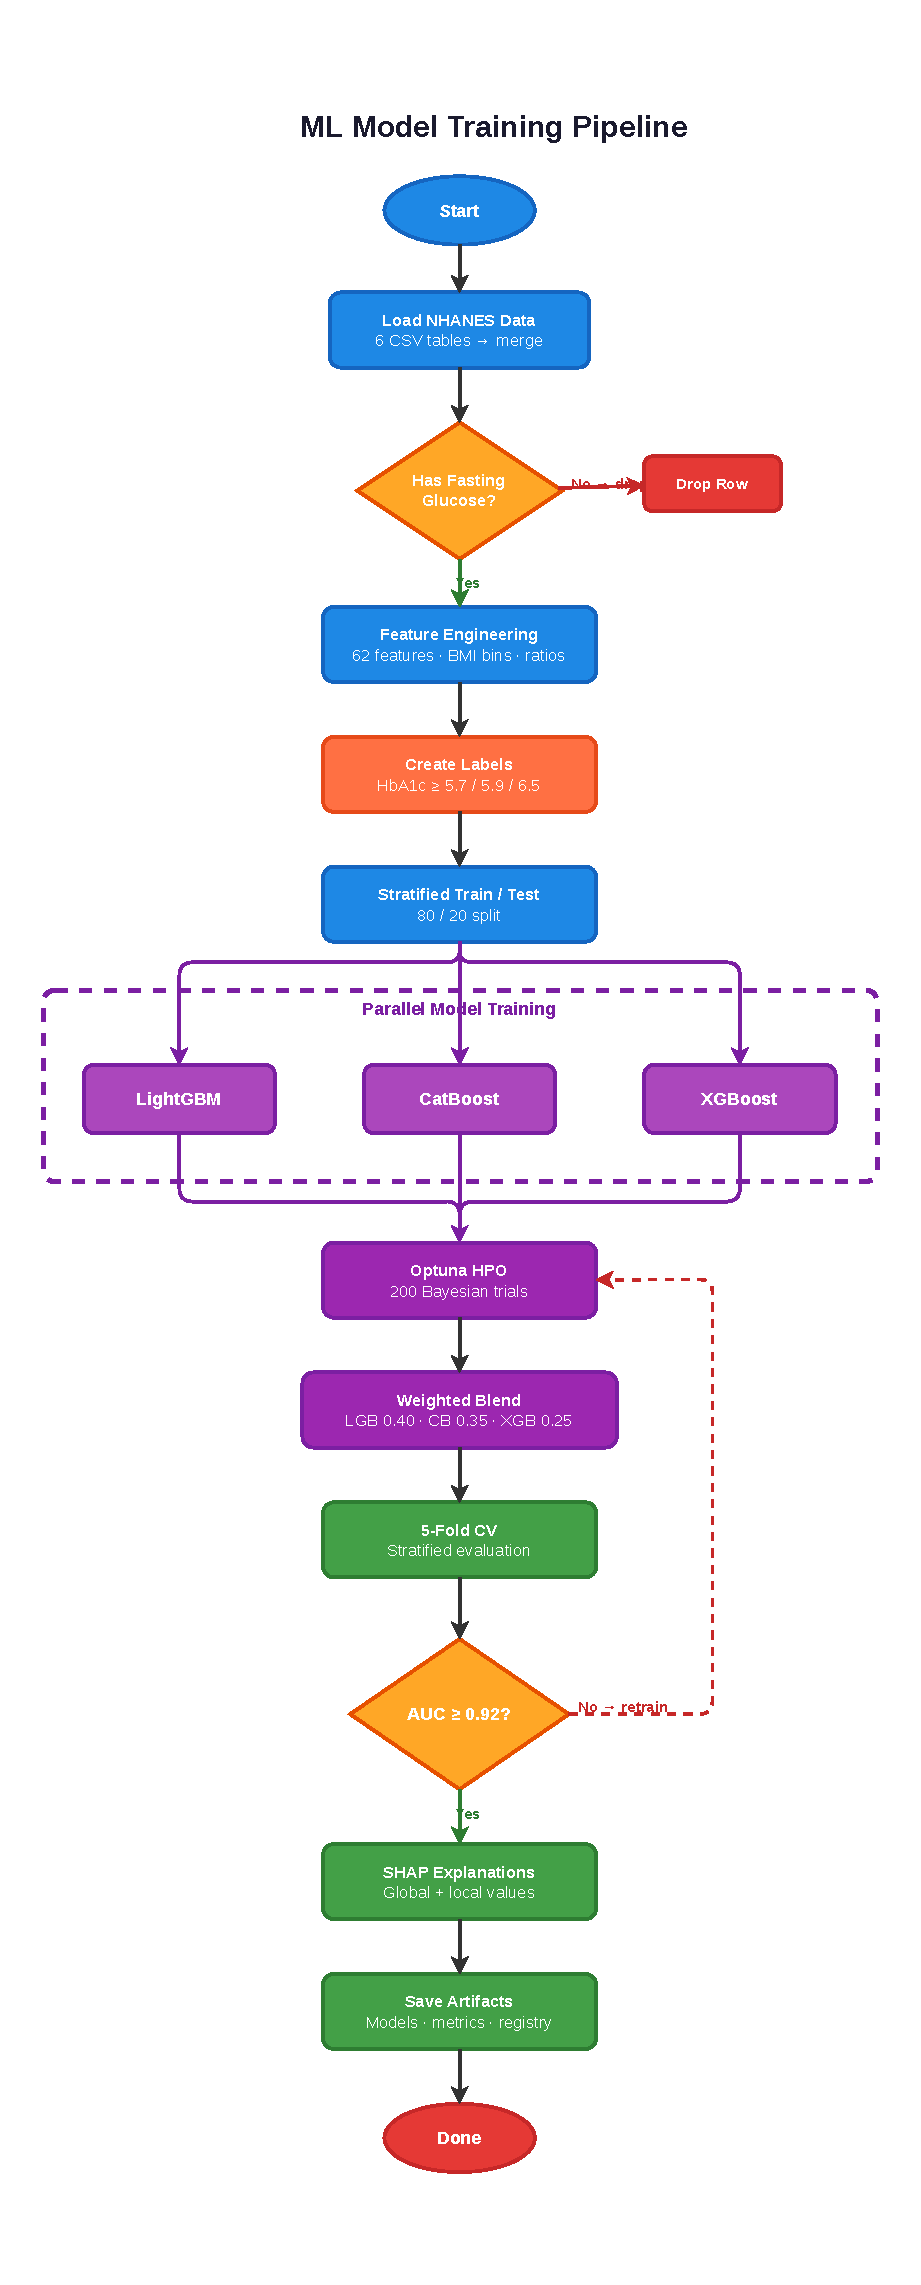
\includegraphics[width=0.92\linewidth, height=4.5cm, keepaspectratio]{Assets/ml_pipeline.pdf}

      \vspace{0.1cm}
      {\scriptsize\textcolor{bodygray}{ML Model Training Pipeline}}
    \end{column}
  \end{columns}
\end{frame}

% =====================================================================
%  SLIDE 13 — Explainability Framework
% =====================================================================
\begin{frame}{Explainability \& Deployment Architecture}
  \small
  \textbf{Three-Tier Explainability Framework:}
  \vspace{0.15cm}

  \begin{columns}[T]
    \begin{column}{0.32\textwidth}
      \begin{block}{\footnotesize Tier 1: Individual-Level}
        \footnotesize TreeExplainer computes exact Shapley values $\to$ per-patient waterfall plots on 12 key features
      \end{block}
    \end{column}
    \begin{column}{0.32\textwidth}
      \begin{block}{\footnotesize Tier 2: Counterfactuals}
        \footnotesize DiCE generates minimal modifiable changes (BMI$\downarrow$, Fiber$\uparrow$, Sleep$\to$7--8\,h) via SHAP-guided search
      \end{block}
    \end{column}
    \begin{column}{0.32\textwidth}
      \begin{block}{\footnotesize Tier 3: Population-Level}
        \footnotesize WHO epidemiological cross-validation verifies feature importance aligns with global diabetes patterns
      \end{block}
    \end{column}
  \end{columns}

  \vspace{0.25cm}
  \textbf{Deployment Stack:}
  \vspace{0.05cm}
  \begin{itemize}
    \setlength{\itemsep}{1pt}
    \item FastAPI\,+\,Uvicorn backend, Next.js~14 frontend, PostgreSQL~18
    \item Docker Compose (6 services), Prometheus\,+\,Grafana monitoring
    \item Fairness auditing module, HIPAA-compliant architecture
  \end{itemize}
\end{frame}

% =====================================================================
%  SLIDE 14 — Section Header: Results & Discussion
% =====================================================================
\sectionslide{Results \& Discussion}{%
 
}

% =====================================================================
%  SLIDE 15 — Results & Discussion
% =====================================================================
\begin{frame}{Results \& Discussion}
  \small
  \begin{columns}[T]
    \begin{column}{0.53\textwidth}
      \textbf{Multi-Threshold Performance:}
      \vspace{0.1cm}

      \renewcommand{\arraystretch}{1.15}
      \centering
      \footnotesize
      \begin{tabular}{l c c c}
        \toprule
        \textbf{Threshold} & \textbf{AUC} & \textbf{CV Mean} & \textbf{Prev.} \\
        \midrule
        $\geq$5.7\% & 0.885 & 0.891 & 35.5\% \\
        \rowcolor{blockbg} \textcolor{accent1}{$\geq$5.9\%} & \textcolor{accent1}{\textbf{0.923}} & \textcolor{accent1}{\textbf{0.923}} & \textcolor{accent1}{24.2\%} \\
        $\geq$6.5\% & 0.972 & --- & 11.0\% \\
        \bottomrule
      \end{tabular}

      \vspace{0.25cm}
      \raggedright
      \textbf{Key Finding:}\\[2pt]
      {\footnotesize AUC increases monotonically with threshold:\\
      \textbf{class separability $>$ model complexity}}

      \vspace{0.15cm}
      \textbf{5-Fold CV Stability:}\\[2pt]
      {\footnotesize Mean AUC = 0.889\,$\pm$\,0.005 \quad Sens.\ = 0.933\,$\pm$\,0.010\\
      Brier = 0.134\,$\pm$\,0.003}
    \end{column}
    \begin{column}{0.45\textwidth}
      \centering
      \vspace{0.1cm}
      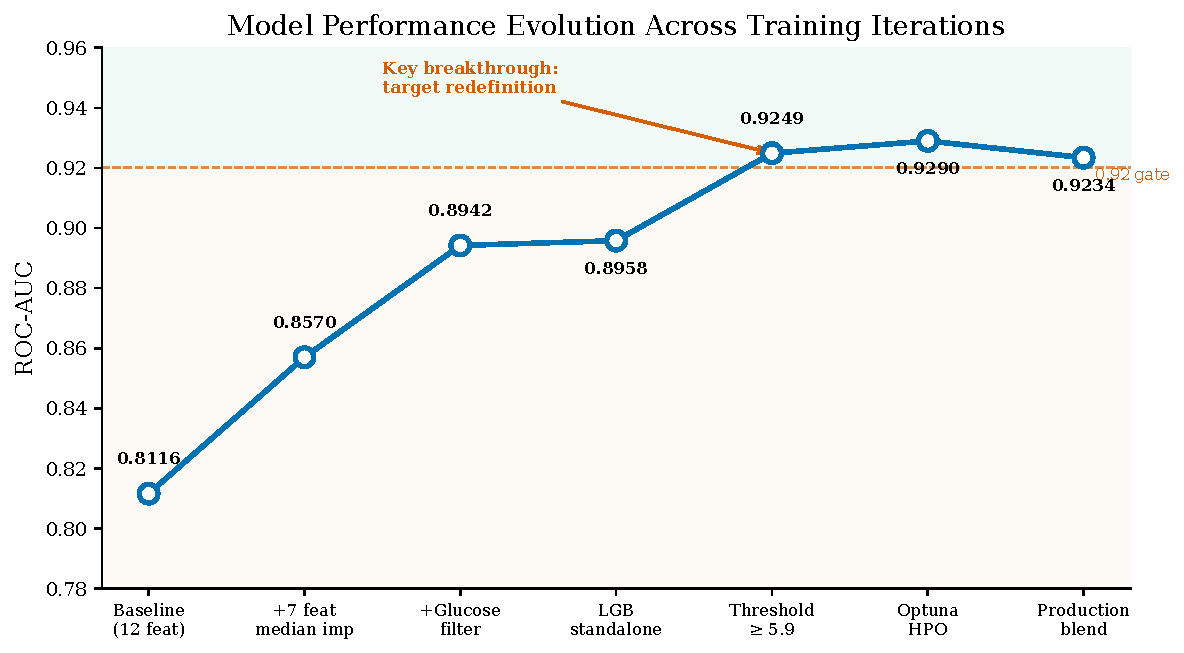
\includegraphics[width=0.92\linewidth, height=4.2cm, keepaspectratio]{Assets/model_evolution.pdf}

      \vspace{0.1cm}
      {\scriptsize\textcolor{bodygray}{Model Evolution: 0.812\,$\to$\,0.923 AUC}}\\
      {\scriptsize\textcolor{bodygray}{Largest gain from threshold sweep (+0.029)}}
    \end{column}
  \end{columns}
\end{frame}

% =====================================================================
%  SLIDE 16 — Section Header: Conclusion
% =====================================================================
\sectionslide{Conclusion}{%
  Key Contributions\\[4pt]
  Limitations\\[4pt]
  Future Work%
}

% =====================================================================
%  SLIDE 17 — Conclusion (Key Contributions)
% =====================================================================
\begin{frame}{Conclusion --- Key Contributions}
  \small
  \begin{enumerate}
    \setlength{\itemsep}{8pt}
    \item \textbf{Multi-threshold design:} Three independent weighted-blend ensembles for HbA1c thresholds $\geq$5.7\%, $\geq$5.9\%, $\geq$6.5\% achieving AUCs of 0.885, 0.923, and 0.972 respectively
    \item \textbf{Threshold dominance discovery:} Target threshold definition --- not model architecture --- is the single most impactful determinant of AUC; largest gain (+0.029) came from threshold sweep, not hyperparameter tuning
    \item \textbf{Three-tier explainability:} Per-patient SHAP waterfall plots, DiCE counterfactual interventions with modifiable features, and WHO epidemiological cross-validation for population-level trust
    \item \textbf{Production-grade deployment:} Full-stack clinical system (FastAPI + Next.js~14 + PostgreSQL~18) with Docker Compose, fairness auditing, Prometheus/Grafana monitoring, and HIPAA-compliant architecture
  \end{enumerate}
\end{frame}

% =====================================================================
%  SLIDE 18 — Limitations
% =====================================================================
\begin{frame}{Limitations}
  \small
  \begin{itemize}
    \setlength{\itemsep}{7pt}
    \item \textbf{Dataset scope:} NHANES is a U.S.-only cross-sectional survey; findings may not generalise to non-Western populations with different dietary patterns, genetic predispositions, and healthcare access
    \item \textbf{Feature ceiling:} HbA1c is excluded from inputs (used as target), so AUC is bounded by the predictive power of non-HbA1c biomarkers --- fundamentally limiting achievable discrimination at $\geq$5.7\%
    \item \textbf{No external clinical validation:} Model was evaluated solely on held-out NHANES data; prospective validation in a clinical setting has not yet been performed
    \item \textbf{Cross-sectional design:} NHANES captures a single time-point; temporal disease progression and longitudinal risk trajectories are not modelled
    \item \textbf{Counterfactual actionability:} DiCE counterfactuals assume independent feature modification, which may not reflect real-world physiological interdependencies (e.g., BMI and blood pressure)
    \item \textbf{Fairness scope:} Demographic parity is audited, but intersectional fairness across multiple protected attributes has not been fully explored
  \end{itemize}
\end{frame}

% =====================================================================
%  SLIDE 19 — Future Work
% =====================================================================
\begin{frame}{Future Work}
  \small
  \begin{itemize}
    \setlength{\itemsep}{6pt}
    \item \textbf{External validation:} Evaluate on non-U.S.\ clinical cohorts (UK Biobank, Indian ICMR datasets) to assess cross-population generalisability
    \item \textbf{Longitudinal modelling:} Incorporate multi-visit NHANES data for temporal risk trajectory prediction using recurrent or transformer architectures
    \item \textbf{Agentic AI integration:} Autonomous follow-up scheduling, adaptive intervention planning, and patient engagement through conversational agents
    \item \textbf{CGM integration:} Fuse continuous glucose monitoring time-series data with survey features using transformer-based deep learning
    \item \textbf{Causal counterfactuals:} Replace association-based DiCE with causal discovery methods (LiNGAM, DoWhy) for physiologically grounded recommendations
    \item \textbf{Federated learning:} Enable multi-institutional model training without centralising sensitive patient data, preserving privacy
    \item \textbf{Personalised thresholds:} Develop patient-specific threshold selection algorithms that adapt screening stringency to individual clinical profiles
  \end{itemize}
\end{frame}

% =====================================================================
%  SLIDE 20 — References
% =====================================================================
\begin{frame}{References}
  \vspace{-0.1cm}
  \scriptsize
  \begin{columns}[T]
    \begin{column}{0.48\textwidth}
      \begin{enumerate}
        \setlength{\itemsep}{0.8pt}
        \item[{[1]}] Khokhar et al., \textit{Artif.\ Intell.\ Med.}, 2025.
        \item[{[2]}] Khalifa \& Albadawy, \textit{Comput.\ Methods Programs Biomed.}, 2024.
        \item[{[3]}] Nie et al., \textit{Heliyon}, 2024.
        \item[{[4]}] Bontha et al., \textit{Appl.\ Sci.}, 2024.
        \item[{[5]}] Tasin et al., \textit{Healthcare Tech.\ Lett.}, 2023.
        \item[{[6]}] Noh \& Kim, \textit{Appl.\ Sci.}, 2024.
        \item[{[7]}] Shah et al., \textit{Sci.\ Rep.}, 2025.
        \item[{[8]}] Prakash \& Subhajini, \textit{IJPRAI}, 2025.
        \item[{[9]}] Maimaitijiang et al., \textit{Healthcare Analytics}, 2025.
      \end{enumerate}
    \end{column}
    \begin{column}{0.48\textwidth}
      \begin{enumerate}
        \setlength{\itemsep}{0.8pt}
        \item[{[10]}] Kabir et al., \textit{Appl.\ Comput.\ Intell.\ Soft Comput.}, 2025.
        \item[{[11]}] Mohanty et al., \textit{PeerJ Comput.\ Sci.}, 2025.
        \item[{[12]}] Prashanthan \& Prashanthan, \textit{Primary Care Diabetes}, 2025.
        \item[{[13]}] Aljaafari et al., \textit{IEEE Access}, 2024.
        \item[{[14]}] Esmaeilyfard \& Bayati, \textit{Sci.\ Rep.}, 2025.
        \item[{[15]}] Acharya et al., \textit{IEEE Access}, 2025.
        \item[{[16]}] Hosseini \& Seilani, \textit{Array}, 2025.
        \item[{[17]}] Lu et al., \textit{Natl.\ Sci.\ Rev.}, 2025.
        \item[{[18]}] Zhu et al., \textit{IEEE Trans.\ Biomed.\ Circuits Syst.}, 2024.
      \end{enumerate}
    \end{column}
  \end{columns}
\end{frame}

% =====================================================================
%  SLIDE 21 — Thank You
% =====================================================================
{%
\setbeamertemplate{headline}{}%
\setbeamertemplate{footline}{}%
\begin{frame}[plain]
  \begin{tikzpicture}[remember picture, overlay]
    % Header bar
    \fill[accent3] ([yshift=0cm]current page.north west) rectangle ([yshift=-0.55cm]current page.north east);
    \node[anchor=west, inner sep=0pt] at ([xshift=0.2cm, yshift=-0.275cm]current page.north west) {%
      \includegraphics[height=0.4cm]{Assets/gbulogo.pdf}%
    };
    \node[anchor=center, text=white, font=\tiny\bfseries] at ([yshift=-0.275cm]current page.north) {%
      Gautam Buddha University \textbar\ School of ICT%
    };
    % Bottom accent line
    \draw[accent1, line width=1.5pt] ([xshift=2cm, yshift=1.5cm]current page.south west) -- ([xshift=-2cm, yshift=1.5cm]current page.south east);
  \end{tikzpicture}

  \vspace{1.5cm}

  \begin{center}
    {\fontsize{32}{40}\selectfont\textcolor{dk2}{\textbf{Thank You}}}

    \vspace{0.6cm}
    {\normalsize\textcolor{bodygray}}

    \vspace{0.5cm}
    {\small Tanya Singh \quad$\vert$\quad 215/ICS/030}\\[4pt]
    {\small\textcolor{accent1}{Gautam Buddha University}}
  \end{center}
\end{frame}
}

\end{document}
